\documentclass[11pt]{scrartcl}
\usepackage[parfill]{parskip}
\usepackage{graphicx}
\usepackage{booktabs}
\usepackage{tabulary}
\usepackage{float}
\usepackage{eurosym}
\usepackage{hyperref}

\graphicspath{{images/}}

\title{\textbf{Economic Aspects}}
\subtitle{Business Model}
\author{Ricardo Garc\'ia Fern\'andez}
\date{\today}

\begin{document}

\maketitle

\vfill

\begin{flushright}
    \copyright  2013 Ricardo Garc\'ia Fern\'andez - ricardogarfe [at] gmail [dot] com.

    This work is licensed under a Creative Commons Attribution- ShareAlike 3.0 License.
    To view a copy of this license visit:
 
    \url{http://creativecommons.org/licenses/by-sa/3.0/legalcode}.
\end{flushright}

\begin{figure}[h]
    \begin{flushright}	
        
\includegraphics{by}
        \label{fig:by-sa}
    \end{flushright}
\end{figure}

\newpage

\tableofcontents

\newpage

\section{Business model}

Business plan for a company in which libre software clearly has an impact. The plan has to be detailed enough. 

Detailed description:

Think about an hypothetical start-up company, with an activity based libre software, or for which libre software may mean a difference. Create a short business plan for 

A previous discussion can be done in groups of up to three persons. Once the discussion has dealt with all the topics, and the plan (or plans) is defined, each student should write her own business plan for it. It should include:

\begin{itemize}
    \item Name of project
    \item Main goals and brief description of the start-up.
    \item License type and overall strategy.
    \item Briefly detail some strategic areas.
    \item Fill in Osterwalder’s canvas, in the following (suggested) order (you don’t have to actually write on the poster, but just include information for each of the following topics):
    \begin{itemize}
        \item Clients segments
        \item Value proposal
        \item Channels
        \item Key resources
        \item Cost structure
        \item Revenues streams.
        \item Customer relationships
        \item Key activities
        \item Key partners
    \end{itemize}
\end{itemize}

\section{Title}

\textbf{IncreaseStack}: IncreaseStack is stack for increase developers productivity. Allows developers to do what they do best, develop. Provides an overview of the project in order to make decisions, improve development and repeat successes in upcoming projects.

\section{Description}

\emph{IncreaseStack} it's a stack of applications for developers that provides a controlled, replicable and scalable for application development. 

\par This stack of applications within the world of IT is known as PaaS (Platform as a Service) and seeks to facilitate application development by providing a familiar environment, controlled, easily expandable and usable to users. All distributed through a server which manages all processes.

\par Start a project is as simple as creating a new project in one place, the management console. The subsequent process is left in the battery that automates and integrates the tedious process of configuring the tools one by one, each time you create a project.

\par The beginin is important, but we all know that the road is much more and we can not forget anything. So IncreaseStack provides constant monitoring of the evolution of the project to take care of all the details and to stress upon which we define as most important.

\par Orchestrated application set comprises:

\begin{itemize}
    \item IncreaseStack - Diagnosis Project Health - Under GPLv3 License (\emph{referenced in section}~\ref{lic:floss}). IncreaseStack porvides information about all data collected in proyect development to generate an analysis for project health and statics per each developer.
    \item SidelabCodeStack - It's a stack of applications for development projects\footnote{http://code.sidelab.es/projects/sidelabcodestack/wiki/SidelabCodeStack} under FLOSS License %TBC.
    It's a stack of applications for development projects including:
    \begin{itemize}
        \item \emph{Management Console} - Centralized project management under GPLv3 License (\emph{referenced in section}~\ref{lic:floss}). A GUI to manage all integrated technologies using a REST API.
        \item \emph{LDAP Directory} - User Authentication using OpenLdap\footnote{http://www.openldap.org/} under 3-clause BSD (\emph{referenced in section}~\ref{lic:floss}). OpenLDAP Software is an open source implementation of the Lightweight Directory Access Protocol.
        \item \emph{Task manager} - Redmine task manager\footnote{http://www.redmine.org/} integration under GPLv2 License (\emph{referenced in section}~\ref{lic:floss}). Redmine is a flexible project management web application. Written using the Ruby on Rails framework, it is cross-platform and cross-database.
        \item \emph{Repository} - Git Distributed Source Code Management\footnote{http://git-scm.com/} (chosen after analysis of multiple repositories, see analysis section) under GPLv2 (\emph{referenced in section}~\ref{lic:floss}). Git is a free and open source distributed version control system designed to handle everything from small to very large projects with speed and efficiency.
        \item \emph{Maven repository} - Archiva Maven Repository\footnote{http://archiva.apache.org/index.cgi} under Apache License v2.0 (\emph{referenced in section}~\ref{lic:floss}).
        Apache Archiva™ is an extensible repository management software that helps taking care of your own personal or enterprise-wide build artifact repository. It is the perfect companion for build tools such as Maven, Continuum, and ANT.
        \item \emph{Application Deployment} - Apache Tomcat\footnote{http://tomcat.apache.org/} under Apache License v2.0 (\emph{referenced in section}~\ref{lic:floss}). Apache Tomcat is an open source software implementation of the Java Servlet and JavaServer Pages technologies. The Java Servlet and JavaServer Pages specifications are developed under the Java Community Process.
        \item \emph{Continuous integration} - Jenkins\footnote{http://jenkins-ci.org/} under MIT License (\emph{referenced in section}~\ref{lic:floss}). An extendable open source continuous integration server.
    \end{itemize}
    \item Email management - VMware Zimbra integration\footnote{http://www.zimbra.com/} - Zimbra Public License (\emph{referenced in section}~\ref{lic:floss}). VMware Zimbra is an enterprise-class email, calendar and collaboration solution, built for the cloud, both public and private. With a redesigned browser-based interface, Zimbra offers the most innovative messaging experience available today, connecting end users to the information and activity in their personal clouds.
    \item \emph{Code quality analyzer} - Sonar\footnote{http://www.sonarsource.org/} under GPLv3 (\emph{referenced in section}~\ref{lic:floss}). Sonar is an open platform to manage code quality. As such, it covers the 7 axes of code quality; Architecture \& Design, Duplications, Unit tests, Complexity, Potential bugs, Coding rules, Comments.
    \item \emph{IDE Integrated Development Environment} - Eclipse (http://www.eclipse.org/) and Eclipse Orion (https://orionhub.org/) using Eclipse Public License (\emph{referenced in section}~\ref{lic:floss}). \emph{Eclipse}; Eclipse is a multi-language software development environment comprising a workspace and an extensible plug-in system. \emph{Eclipse Orion}; Orion's objective is to create a browser-based open tool integration platform which is entirely focused on developing for the web, in the web.
    \item Migration Guide and integration of existing projects to stack.
    \item Ability to integrate new technologies into the application stack.
\end{itemize}

\par \emph{IncreaseStack} gives the opportunity to rule them all. We focused development process around Java development. After studing most demanded and used programing languages, the most complete solution has to be in Java. Seeking information on the most popular programming languages​​, we find this chart in a job search portal, Infojobs\footnote{http://orientacion-laboral.infojobs.net/competencias-mas-demandadas-informatica-telecomunicaciones}.

\begin{figure}[htp]
\begin{center}
  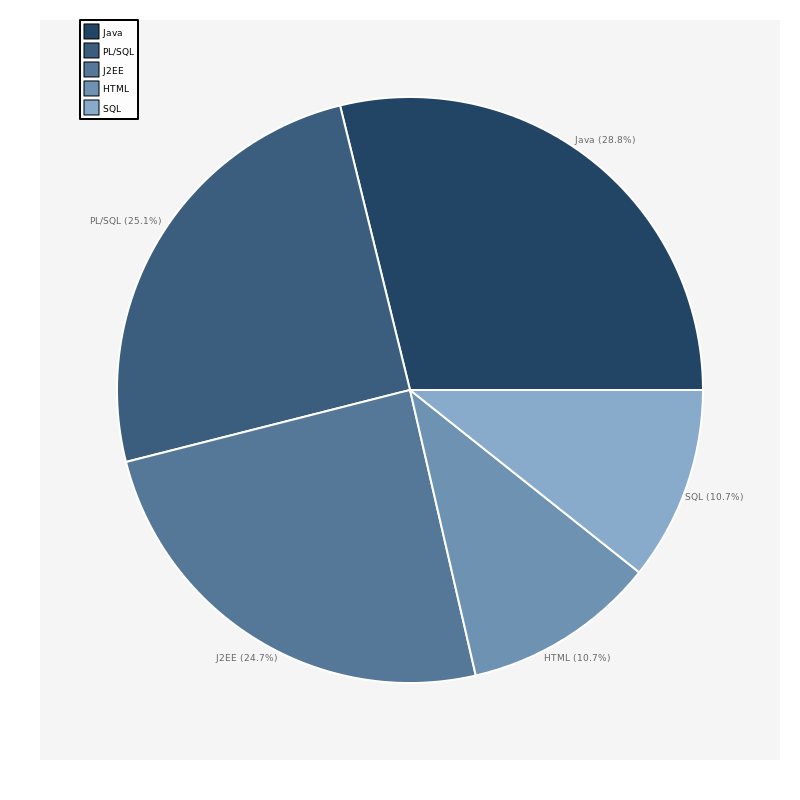
\includegraphics[width=0.7\textwidth]{images/requested-programming-language-piechart.png}
  \caption{Software Development most required languages}
  \label{fig:req-languages}
\end{center}
\end{figure}

\par In another analysis by Tiobe index\footnote{http://www.tiobe.com/index.php/content/paperinfo/tpci/index.html} regarding languages ​​used by the community. We see Java in second position, with 17.417\% of the market, following C with 17.855\%. A little difference between the most used languages.

\par Therefore we focused \emph{IncreaseStack} in Java.

\par This set of applications provides a record of precious information for the development of projects because we are able to know the status of each project developed by a metric defined in order to know what we do well and where we need to improve as a development team.

\par The solution we provide, if we do not work is useless. IncreaseStack brings more quality is through the mentoring program to take advantage of these tools for both developers and the management and health of projects.

\par So by studying the data stored in the records of each of the applications provide centralized state analysis total project and its developers through IncreaseStack tool. The work is reflected in graphs where you can see the evolution of the repository, managing tasks, each project roadmap, developments and code quality of each role. Our utopia points in the direction of efficient management of resources educating them to learn from our successes and our mistakes follow a growing line of evolution in application development.

\par \emph{This is the point that leads to the Utopia, learning from our past.}

\section{Organization}

\par In our company we aim, \emph{utopia in application development}. Utopia means not leaving to pursue an idea, take the idea forward and forever realize that the more we walk further away. That means we're doing our job, because we keep thinking and discovering that something better is yet to come. This feeling is more real in the field of IT so we have thrown our little utopia, the integration of tools for software development with IncreaseStack.

\par To provide everything a developer needs to only focus on developing. Thus we approach the standards in application development.

\par The complete application stack consists of FLOSS tools established as standards in their respective niche markets. We chose these tools because we could evaluate, its impact, its use, around existing projects and user reviews.

\par The development community FLOSS applications grows exponentially as a use in all fields, not just in IT.

\par In the field of IT use FLOSS tools facilitates access to power that leaves our hands. We through that power, which is so easily accessible today, in which we have based our product to focus our efforts on providing solutions to development teams in their daily lives. We built on standards, so do not depend on a particular technology to keep evolving. \emph{Interoperability is our greatest asset, we are experts in communication.}

\section{Osterwalder's model}

\par We can translate the project according to the business model canvas of Osterwalder.

\subsection{Clients segments}

This software solution is aimed at small, medium businesses and developers. The unification of the tools to generate quality software is increasingly valued by the search for efficiency, best practices and standardization in the development of software. The health of the projects plays an important role in the development of software and comprehensive analysis of the source code represents a substantial improvement. We all know that it is very difficult to manage thousands and thousands of lines of code, so that by automating resource standard and is much easier to obtain reports on software quality.
    
\subsection{Value proposal}

\par The added value offered by us for IncreaseStack, is that through the use of standards for the development, speeding up the time of commissioning and project management. Moreover, the collection of tools that generate information about a project (repository, issues, CI, code quality) and subsequent transformation into human readable reports us apart from other unified solutions as such as Heroku PaaS, CloudFoundry in exposed the summary results.

\par Delving beyond the product, our solution is free and can therefore be evolving through community and other clients that use it. By the cost savings, consolidation and management applications stack, being FLOSS, significant cost savings for the customer at the time of providing tools to its developers. The reporting tool is a FLOSS solution, by managing standards and metrics related to the quality of an application, aims to become a repository of repositories (RoR). In this RoR what we want is a healthy competition between projects, ie a meritocratic competition to see which project is the healthiest, most professional and prepared all staying there

\subsection{Channels}

\par \emph{IncreaseStack} tool is based on the quality and interoperability therefore their environment is the Internet. Internet as such, is more focused on generating FLOSS project analysis to demonstrate its effectiveness. The pilot implementation in several companies and use it to give users.

\par Implementing \emph{IncreaseStack} comes through various channels, the installation on the same server of the company, generating a virtual image to test it on any computer in 10 minutes downloading the project source. All this material is available from the project website with documentation regarding the user and the developer.

\par The source code is hosted on github (the development and stable versions) that is a mirror of the company's own repository. \textbf{Social Marketing Source Code}.

\par Universities are the pillars of the knowledge management are the main producers of knowledge. Experimientación are open to and part of his job (of teachers) is innovation. So it is a very important channel for disseminating IncreaseStack.

\subsection{Key resources}

\par As key resources begin by IncreaseStack tool developers. Experts in data mining and database analysis.

\par Also be included as key resources, pilot tests in universities, conferences, lectures, specialist websites. All this from the inside out, an expansive advertising.
\par Reporting the results produced by other tools FLOSS tool known. As a summary and general idea, a community inclusion to make a spark of curiosity.
    
\subsection{Cost structure}

\par Cost to produce the product. Material. Relevant costs. If the differential saves FLOSS be mentioned specifically. Dividing the cost structure we can see:

\par The IncreaseStack platform development. It takes a group of 3 full time dedicated developers. Let's say the first version out in six months and prepared for analysis com pilot project implementation. This becomes.

\par \emph{FLOSS}, through the use of FLOSS tools get all the necessary resources and integrate, we have a 0 cost. The base course, because we can use development is being done in SidelabCode Stack. It would require integrating:

\begin{itemize}
    \item Sonar code analysis.
    \item Zimbra Mail client.
    \item Eclipse and Eclipse Orion.
    \item IncreaseStack as a tool for the analysis of the data we have available.
\end{itemize}

\par So we've gone from having to develop or pay for 11 applications to integrate management and development 3 and develop a respect to the analysis produced by the use of the other.

\par The initial cost is divided into the following groups:

\begin{itemize}
    \item Developers
     By using the basic \textbf{COCOMO} model equation\footnote{http://www.sc.ehu.es/jiwdocoj/mmis/cocomo.htm}  as organic project.

    E = Effort KLDC b = a (person x months)
    
    T = Time duration of development effort d = c (months)
    
    E / T = month

    \begin{table}[H]
        \centering
        \begin{tabular}{|l|l|l|l|}
            \hline a & b & c & d\\
            \hline 1.05 & 2.4 & 2.5 & 0.38\\
            \hline
        \end{tabular}
    \end{table}

    \item Hardware for Developers: 4.000\euro in PC.
\end{itemize}

\par Assuming that contains 4000 lines of code (4 in KLDC) and taking into account that this is a project for two estimated a duration of 3.81 months.
\par The average salary of a software developer is estimated at 26719\euro\footnote{http://empleo.trovit.es/salarios/programador-software} so the investment would 17812.6\euro.
    
\par A \textbf{total cost of 21812,6\euro}. With a simple inverse proportion between the cost of 4 proyects integration against 11, we have as a result: 59984,65\euro. Develop the other projects will cost much more. I know these numbers are not real but what I find is the savings you get. With numbers closer to reality (lines of code for all projects) the difference would be at least 5 times.

\par The investment analysis focuses on a person in charge of converting the data to human language. We have to invest 12000\euro on that person for the initial product is ready in six months. This cost doesn't depend on FLOSS.

\par Total initial amount of 33812,6\euro.

\subsection{Revenues streams}

\par How to recover the capital that has been invested?

\par We follow an ascending line in implementing working methods. By analyzing the reliability of collected and publicized it creating a RoR to give a solid feel. Thus by implementing IncreaseStack and classroom training courses we can estimate that the initial capital invested will be recovered in two years. Is the deadline and a very important date with respect to the average life of enterprises.

\par Income/Expenses. The initial costs are favored by the use of FLOSS applications in a huge as seen above. Therefore, we must build on that initial investment in order to increase the quality of service we provide. The revenues come from the hand of the implementation in companies IncreaseStack (59,984.65\euro in development cost and 12000\euro in analysis). We want to be functional in two years in a number of 30 companies. If we reach this number we can continue expanding and offering better solutions.

\par The cost of implementation is 'apparently' simple 33812,6\euro / 30 = 1127.08\euro. An expense for a company derisory compared with the facilities that can provide IncreaseStack the development of their applications. We get money from the sale of \emph{IncreaseStack}, doubling the price. 1000\euro is no money for a company so we thought of selling the solution for 2000\euro, to get its money and make a profit in order to continue improving as developers. Using the numbers obtained for the \emph{30 companies in two years} we can see the result: 30 * 2000 = 60000\euro.

\par We know that spending per year will not be 33812,6, will be greater. But we are sure that we can recover the initial expense in this time comfortably and in a year, make a profit.

\subsection{Customer relationships}

\par How to access the customers? if they exist in your contacts, get publicity, etc.. If incorporated or not the product development as a community.

\par Access to customers or partners be done through the use of key resources, universities, business and industry related online communities.
Access to universities through presentations of the idea in the IT related departments. Showing as well, our main goal, the utopia of standards and quality improvement in the developments.

\par For enterprises, knowing this world where everything is closer than it seems, we can always introduce our project known companies, known to us not by the brand company, in which we have worked and circles of friends own dedicated to this sector. Always bear in mind make or break a spark for collaboration. Never think that it is essential IncreaseStack, IncreaseStack helps improve.

\par Interaction with customers. In this section we engage with clients to believe they perceive that the solution we have created. We must maintain a good communication and be open-minded in order to improve all that's what it is. We have to turn customers into collaborators, not for a tailored solution if not for a solution tailored to many more people, ie standardize procedures by existing market standards.

\par 
\begin{itemize}
    \item Corrección de ejercicios, examen, meritocracia en cursos aprobados. Fidelización de clientes.
\end{itemize}

\subsection{Key activities}

\par How to access the customers? if they exist in your contacts, get publicity, etc.. If incorporated or not the product development as a community.

\par Interacting with customers. It may not be interesting to keep in touch with your customers.

\par Keys to the business, to publicize the product, development, etc.
\begin{itemize}
    \item Include and encourage the development and use in university by students and teachers.
    \item Implementation of pilot programs in companies.
    \item Building community through the use of the product. Standardizing metrics, working methodologies, training courses, tutorials and certify knowledge through partnerships with communities of each of the different products. Also a good advertisement campaign.
    \item Promote use and results: Studies and documents supporting the results unlike the use of the product. As be applied to increase efficiency in application development.
\end{itemize}

\subsection{Key partners}

\par Partners, people helping the marketing and development. Partner is anyone who works in a business. We aim to turn customers into partners.

\par Applying this definition we intend to turn customers into partners and involve the university, so that in this way give rise to a community that may be governed by its own rules.

\section{How FLOSS influenced my model}

\par FLOSS is not only the means by which the end is achieved, is the end in itself as well.

\par Without FLOSS, this project would never exist. So what are we to FLOSS, so also is the end in itself. It is a circular flow of power to the entire world, where we give and receive, ie shared, innovative and above all, it helps.

\par FLOSS need if we are to grow, if we standardize the product, adopt new technologies, new fields (not just IT) and keep in line with the standards created through debate among the users themselves.

\par FLOSS gives us a consensus between communities (companies, users, developers, universities) in which no one, no one above, makes the rules, everyone can contribute, suggest, ask.

\par Through the exercise of reason, consensus is reached and this is what is reflected in FLOSS projects, above all, is what we call the common good or best practices (IT terms).

\section{Further Work}

\par As improvements in \emph{IncreaseStack} solution:

\begin{itemize}
	\item Standardization of software quality. 
	\item Different installations for developing with other programing languages.
\end{itemize}

\section{FLOSS Licenses}\label{lic:floss}

This is a list of FLOSS licenses used in the tools of our product, and of course the license of IncreaseStack\emph{Apache License version 2.0}.

\begin{itemize}
    \item OpenLdap - 3-clause BSD - http://www.openldap.org/software/release/license.html
    \item GNU GPLv2 - GNU GENERAL PUBLIC LICENSE v2- http://www.gnu.org/licenses/old-licenses/gpl-2.0.html
    \item GNU GPLv3 - GNU GENERAL PUBLIC LICENSE v3 - http://www.gnu.org/licenses/gpl.html
    \item Zimbra Public License - http://www.zimbra.com/license/zimbra-public-license-1-3.html
    \item Apache License version 2.0 - http://www.apache.org/licenses/
    \item MIT License - http://opensource.org/licenses/MIT
    \item EPL - Eclipse Public License - http://www.eclipse.org/legal/epl-v10.html.
    \item GNU Affero General Public License - AGPLv3 - http://www.gnu.org/licenses/agpl-3.0.html
\end{itemize}

\end{document}
